\chapter{Clasificación con redes neuronales}
\label{chap:Clasificacion con redes neuronales}
\Abstract{El presente capítulo describe de forma detallada el proceso de análisis de imágenes mediante clasificadores basados en redes neuronales. Se explica de forma detallada el proceso de creación de los clasificadores y se muestra sus capacidades.}

Los clasificadores son redes neuronales diseñadas con el objetivo de identificar. Estas son capaces de indicar si un objeto está en una imagen o no. En este proyecto identificar los objetos no es suficiente ya que también hace falta localizarlos. A pesar de ello, primero se van a entrenar dos clasificadores con el objetivo de que sirvan como base para el desarrollo de los detectores de objetos basados en técnicas one-shot (\autoref{chap:Segmentacion con redes neuronales}).

Por falta tanto de datos como de cálculo computacional, se va a partir de dos clasificadores ya entrenados y se van a reentrenar. Esto proceso es conocido como aprendizaje por transferencia y es ampliamente usado al trabajar con redes neuronales. De esta forma podemos partir de dos clasificadores con estructuras ampliamente corroboradas a la vez que se consigue reducir la carga computacional y con ello el tiempo de entrenamiento. Además, estos clasificadores ya han sido entrenados para la extracción de características lo cual ayudará al sistema a pesar del poco tiempo de entrenamiento. Para llevar a cabo el reentrenamiento primero se han descongelado las capas de convolución para permitir así el aprendizaje. Los dos clasificadores elegidos para ser reentrenados son AlexNet y VGG-16. Los motivos de su elección son: Se caracterizan por redes simples y directas lo cual facilita su comprensión y el trabajo con ellas. Reflejan la evolución de las redes neuronales durante los últimos años. Los dos nuevos clasificadores han sido nombrados como LEGONet y LEGO16 respectivamente. De ahora en adelante se referirá a ellos de esta forma.

\section{Condiciones de entrenamiento}
\label{sec:Condiciones de entrenamiento}
Para poder reentrenar dos clasificadores basados en redes neuronales es necesario disponer de una buena base de datos de la que puedan aprender. Para ello se ha empleado el conjunto de imágenes clasificadas por Intel \citep{IntelDataset}, el conjunto de imágenes de LEGOS clasificadas por Joost Hazelzet \citep{LEGODataset} y el conjunto de imágenes de LEGOS clasificadas por Francisco García \citep{LEGODataset2}. Con la ayuda de estas bases de datos se dispone de un total de 7 clases sobre las que entrenar y un total de 16.398 imágenes de alta resolución. En la \autoref{tab:LEGONet imagenes} se puede ver un resumen de las imágenes usadas. Y en la \autoref{fig:LEGONet montage} se pueden ver algunos ejemplos de las imágenes empleadas para el entrenamiento. Se ha decido emplear la base de datos de Intel ya que disponía de imágenes de alta resolución y al contar con varias estructuras, edificios y calles se dispone de numerosas imágenes con ángulos rectos y secciones. Característica en común con las piezas de LEGO. 

\begin{table}[ht]
  \centering
    \begin{tabular}{|l|r|}
    \hline
    \multicolumn{2}{|c|}{Total de imágenes}\\
    \hline
    LEGOS & 2464 \\
    \hline
    Edificios & 2191 \\
    \hline
    Bosques & 2171 \\
    \hline
    Glaciares & 2404 \\
    \hline
    Montañas & 2512 \\
    \hline
    Océanos & 2274 \\
    \hline
    Calles & 2382 \\
    \hline
    \end{tabular}%
    \caption{Base de datos para el entrenamiento de clasificadores}
  \label{tab:LEGONet imagenes}%
\end{table}%

\begin{figure}[ht]  %LEGONet montage
	\centering
	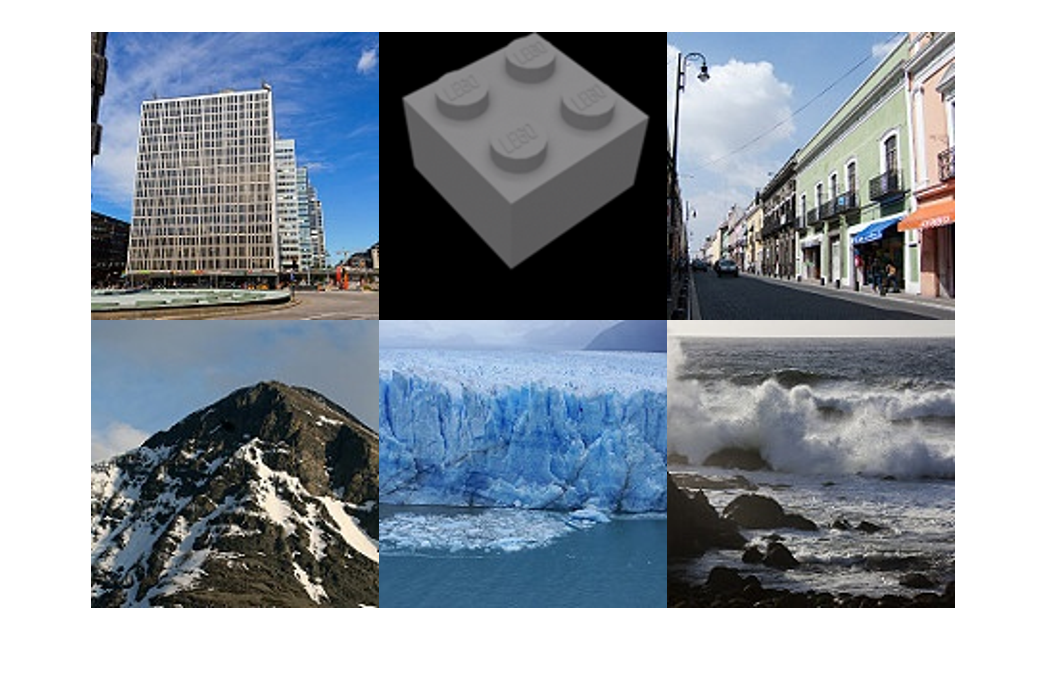
\includegraphics[width=0.5\textwidth]{Classificacion con redes neuronales/montage.png}
	\caption{Muestra de imágenes para el entrenamiento de clasificadores}
	\label{fig:LEGONet montage}
\end{figure}

Todo el entrenamiento se ha llevado a cabo en un ordenador personal equipado con un i7 4790K, 16GB de memoria RAM y una tarjeta gráfica Nvidia Geforce GTX970 con 4GB de VRAM. Teniendo en cuenta las limitaciones por \textit{hardware} y tiempo, se han realizado múltiples entrenamientos con diferentes opciones de entrenamiento para obtener los mejores resultados con cada red.

\section{LEGONet}
Originalmente AlexNet fue diseñado para trabajar con la base de datos de ImageNet, que cuenta con más de 14 millones de fotos y 1000 clases diferentes. Para este proyecto se ha decidido reentrenar esta red neuronal con imágenes de LEGOS para mejorar su reconocimiento de estos y así usarla posteriormente como base para los detectores de objetos. Por ello, con la ayuda de MATLAB y del conjunto de imágenes clasificadas por Intel \citep{IntelDataset}, el conjunto de imágenes de LEGOS clasificadas por Joost Hazelzet \citep{LEGODataset} y el conjunto de imágenes de LEGOS clasificadas por Francisco García \citep{LEGODataset2} se ha reentrenado AlexNet para clasificar un total de 7 clases diferentes.

\subsection{Estructura}
En el 2012, AlexNet se caracterizó por ser una red neuronal muy grande y pesada para la época. Está formada por 60 millones de parámetros y un total de 650.000 neuronas. Al contrastarlo con sistemas actuales puede no parecer tan grande, pero dada la época y las limitaciones por hardware para entrenarla, fue un gran salto. La estructura de la red se divide en 5 capas convoluciones y dos capas completamente conectadas. Las capas convolucionales se unen entre si con capas \textit{Relu}, \textit{Batch normalization} y \textit{Max Pooling}. Las capas de activación \textit{Relu} se usan para evitar la presencia de valores nulos y negativos que puedan entorpecer el aprendizaje, su función es $ReLu = max(0,x)$ (ver \autoref{fig:ReLu}) \citep{ReLu}. Existen múltiples funciones de activación además de \textit{Relu}, pero esta es altamente usada, ya que apenas supone carga computacional y permite que en grandes redes, los errores se puedan propagar y las capas más profundas puedan aprender. \textit{Batch normalization} tal y como su nombre indica, regulan  y normalizan el aprendizaje de forma que evitan un aprendizaje repentino y brusco y reducen la posibilidad de un sobreaprendizaje. Además, permiten que las capas aprendan de forma independiente del resto de la red agilizando así el entrenamiento. Y por último, las capas \textit{Max Pooling} se emplean para reducir las dimensiones de las capas intermedias y contener así a las red neuronal.

Las capas completamente conectadas están también conectadas entre sí con capas \textit{Relu} y \textit{dropout}. Las capas \textit{dropout} sirven para evitar el sobre aprendizaje, es decir, evitar que la red se aprenda los casos en lugar de las características. Para ello lo que se hace es que todas las neuronas tienen una probabilidad previamente establecida de ser desconectadas. En AlexNet esta probabilidad es del 50\%. De esta forma se controla el sobre aprendizaje.


\begin{figure}[ht]  %ReLu
	\centering
	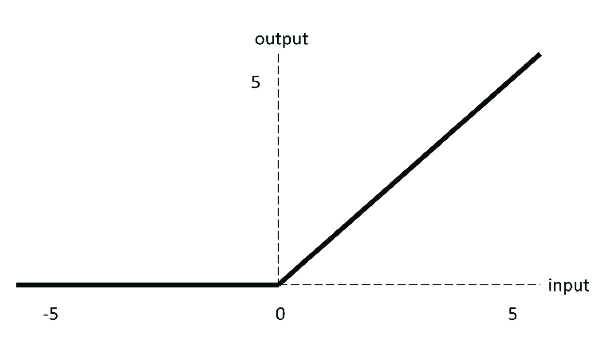
\includegraphics[width=0.7\textwidth]{Classificacion con redes neuronales/ReLu.png}
	\caption{Funcionamiento de \textit{Relu}(Rectified Linear Unit)}
	\label{fig:ReLu}
	\vspace{-5pt}
\end{figure}


Para reentrenar AlexNet con las nuevas clases es necesario modificar lo ya que este ha sido diseñado para reconocer 1000 clases en lugar de 7. EL primer paso consiste en el descongelamiento de las capas de convolución para que así la red pueda aprender. A continuación, es necesario eliminar las tres últimas capas que se encargan de la clasificación y sustituirlas por capas similares, pero de una correcta dimensión para detectar las siete clases. Los cambios a aplicar son:
\begin{itemize}
\item Capa 23: Completamente conectada (1x1x1000) $\rightarrow$ (1x1x7)
\item Capa 24: \textit{Softmax} (1x1x1000) $\rightarrow$ (1x1x7)
\item Capa 23: Salida clasificador
\end{itemize}

A continuación se muestra la estructura final en la \autoref{fig:LEGONet} y la activación de la primera capa convolucional en la \autoref{fig:LEGONet conv}.
	
\begin{figure}[ht]  %LEGONet
	\centering
	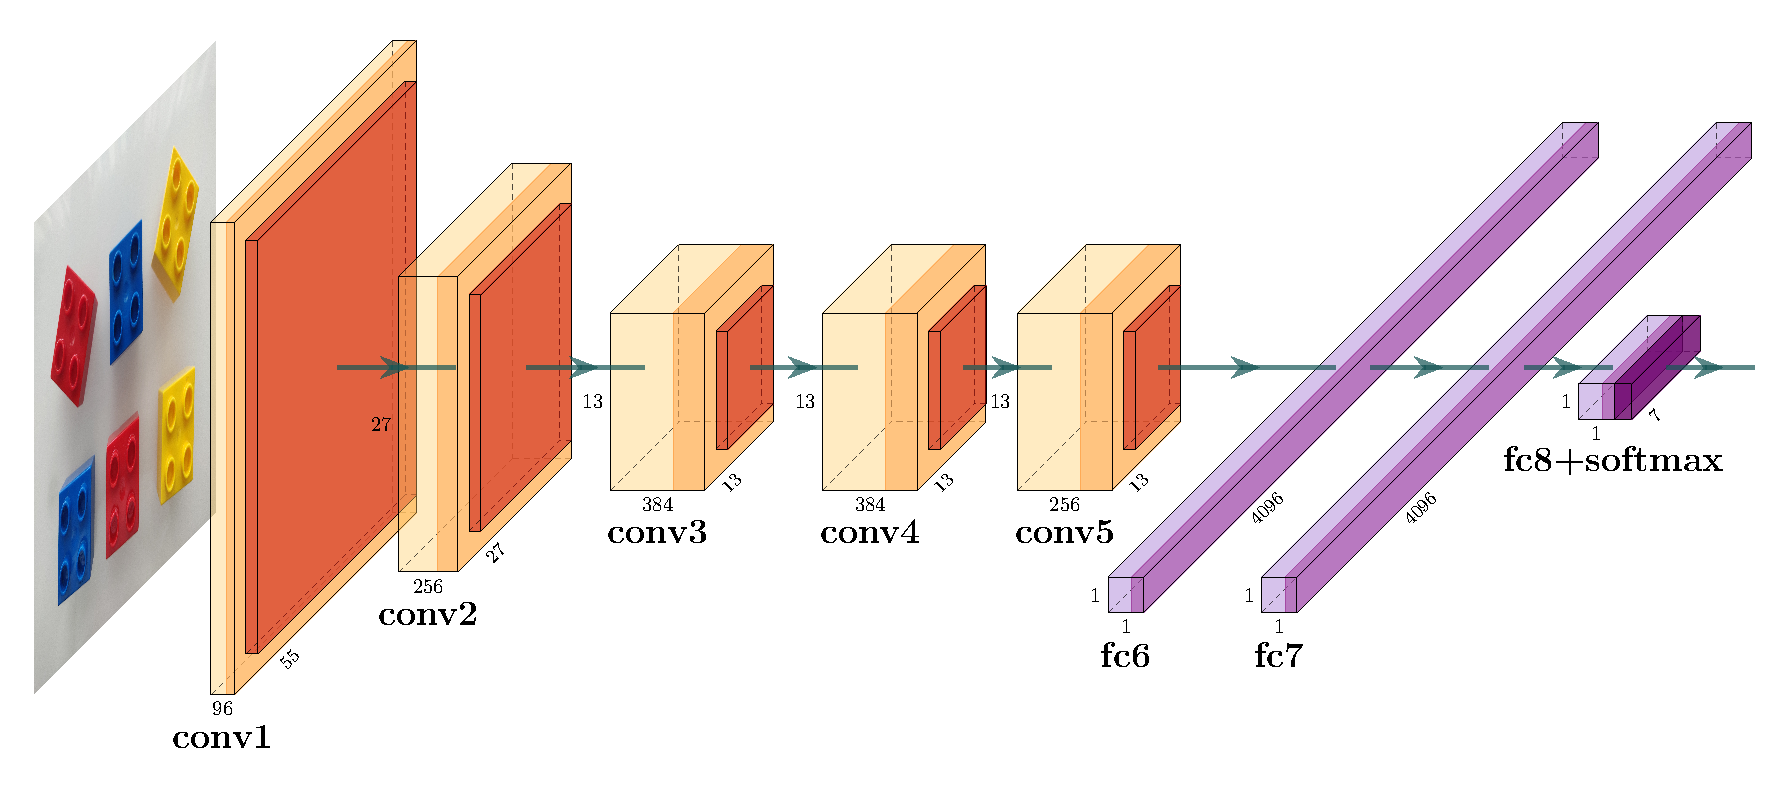
\includegraphics[width=0.95\textwidth]{Classificacion con redes neuronales/LEGONet.pdf}
	\caption{Estructura de LEGONet}
	\label{fig:LEGONet}
\end{figure}

\begin{figure}[ht]  %LEGONet conv
	\centering
	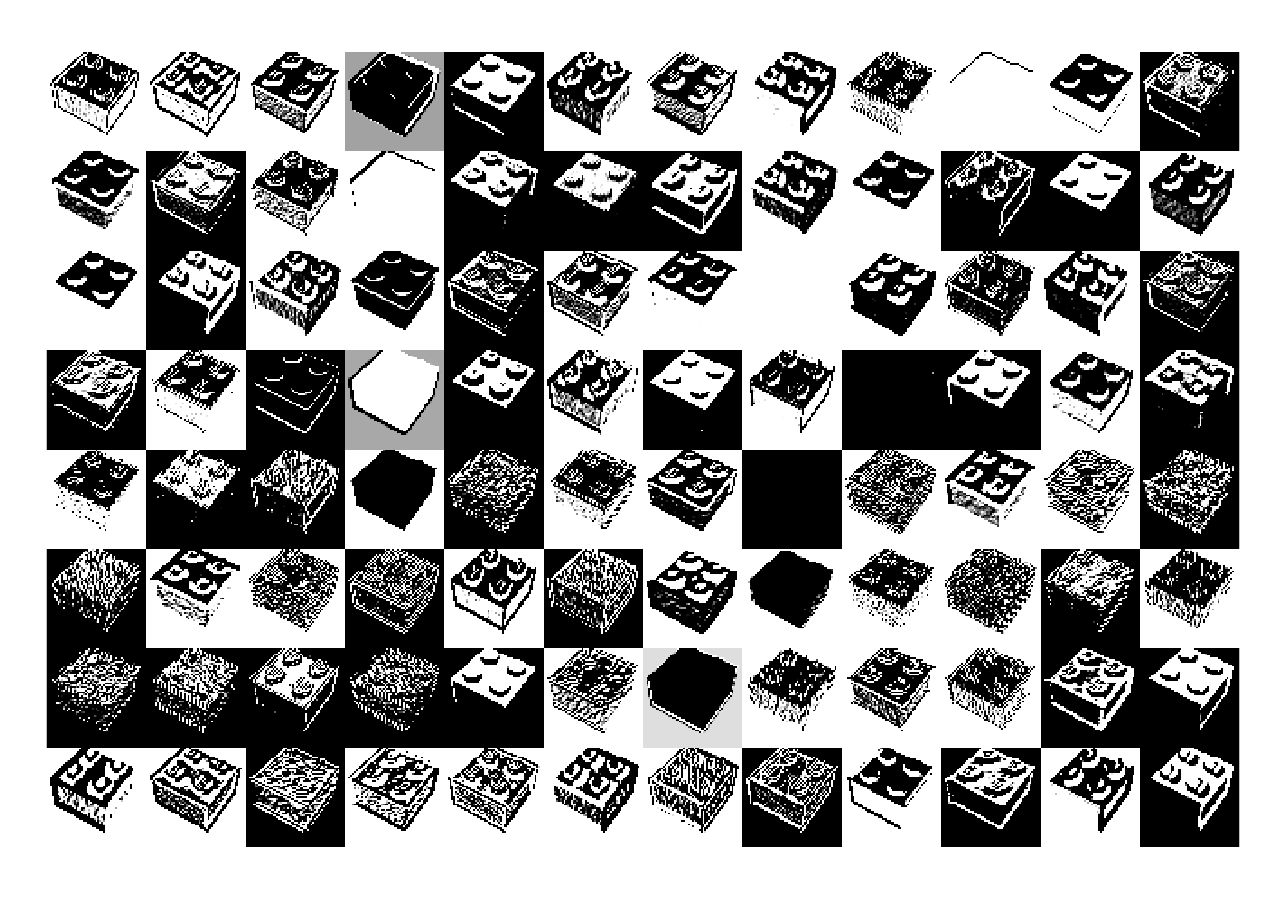
\includegraphics[width=0.7\textwidth]{Classificacion con redes neuronales/LEGONet_conv1.png}
	\caption{Activación primera convolución de LEGONet}
	\label{fig:LEGONet conv}
\end{figure}


\subsection{Entrenamiento}
\label{subsec:Entrenamiento LEGONet}
Con la ayuda de MATLAB y del conjunto de imágenes elaborado en \autoref{sec:Condiciones de entrenamiento} se ha reentrenado a AlexNet para identificar 7 clases. Tras numerosas pruebas se han seleccionado las opciones de entrenamiento mostradas en la \autoref{tab:LEGONet options}.

\begin{table}[ht]
  \centering
    \begin{tabular}{|l|c|}
    \hline
    \multicolumn{2}{|c|}{Opciones de entrenamineto} \\
    \hline
    Solver & \multicolumn{1}{l|}{Stochastic Gradient Descent with Momentum (SGDM)} \\
    \hline
    Momentum & 0.9 \\
    \hline
    Initial Learn Rate & 1.00E-04 \\
    \hline
    Learn Rate Schedule & piecewise \\
    \hline
    Learn Rate Drop Factor & 0.1 \\
    \hline
    Learn Rate Drop Period & 5 \\
    \hline
    L2Regularization & 0.004 \\
    \hline
    Max Epochs & 30 \\
    \hline
    Mini Batch Size & 128 \\
    \hline
    Shuffle data & every epoch \\
    \hline
    \end{tabular}%
  \caption{Opciones de entrenamiento de LEGONet}
  \label{tab:LEGONet options}%
\end{table}%

\subsection{Resultados}
Con la ayuda de MATLAB y de las bases de datos previamente comentadas, se va a realizar una evaluación del clasificador. En total se han empleado más de 3000 imágenes y a continuación se muestran los resultados obtenidos en forma de matriz de confusión (ver \autoref{fig:matriz LEGONet}).

Analizando estos resultados se puede obtener las tasas de acierto y tasas de fallo y si se realiza un estudio más intensivo analizando los verdaderos positivos y los falsos positivos (ver \autoref{fig:ROC LEGONet}). Este tipo de representación se conoce como curva \textit{ROC} (\textit{Receiver Operating Characteristic} o Característica Operativa del Receptor) y es ampliamente usada al evaluar clasificadores ya que permite mostrar de forma gráfica el comportamiento de la red. Otro dato importante de esta curva es el área que encierra, este dato es conocido como \textit{AUC} (\textit{Area Under the Curve}) y es muy representativo de las capacidades de la red para identificar. Este dato se puede ver en la \autoref{tab:ROC LEGONet}.

Las tasas de acierto y las ACUs obtenidas es bastante elevada si se tiene en cuenta el poco tiempo de entrenamiento y las circunstancias dadas. Si nos fijamos solo en los LEGOS observamos que los resultados son incluso mejores ya que no ha habido ninguna pieza mal identificada y solo se han identificado mal como LEGOs tres imágenes. Es decir, una tasa de acierto al identificar LEGOS del 100\% y una tasa de falsos positivos para LEGO del 0.7\%.

\begin{figure}[ht]  %Matriz LEGONet
	\centering
	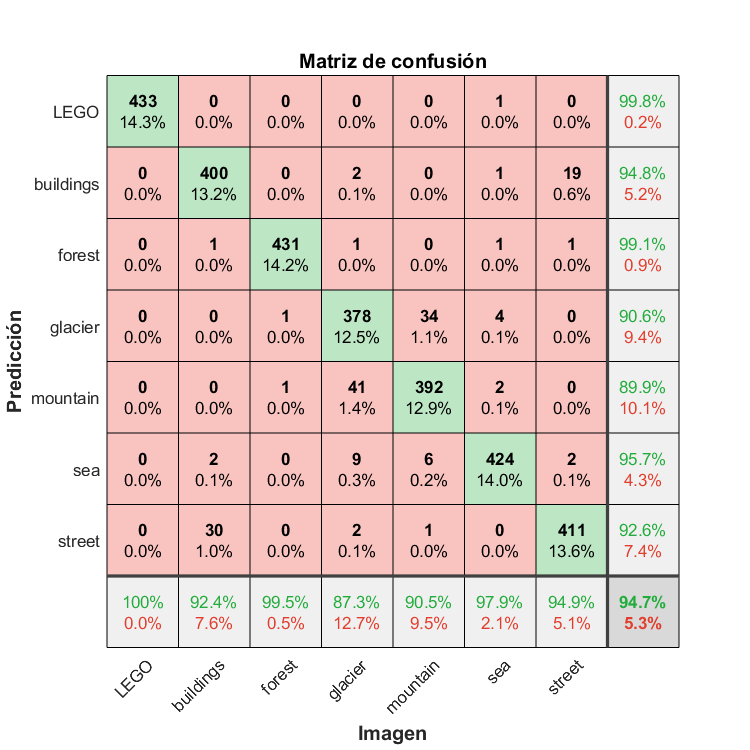
\includegraphics[width=0.8\textwidth]{Classificacion con redes neuronales/LEGO16_matriz.png}
	\caption{Evaluación de LEGONet: matriz de confusión}
	\label{fig:matriz LEGONet}
\end{figure}

\begin{figure}[ht]  %ROC LEGONet
	\centering
	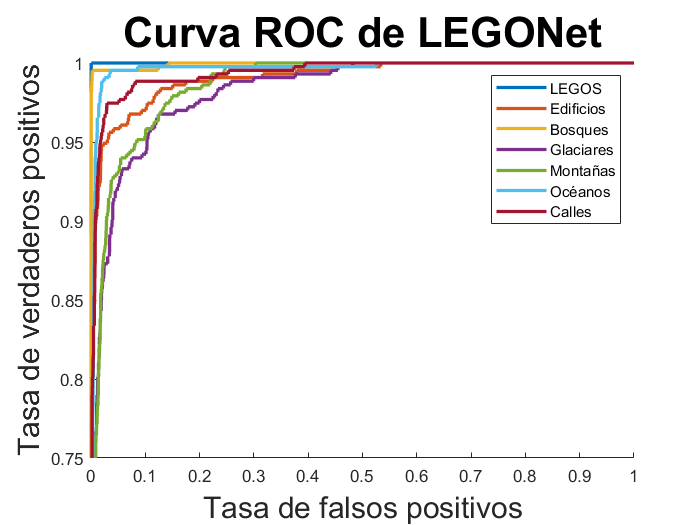
\includegraphics[width=0.8\textwidth]{Classificacion con redes neuronales/ROC2 LEGONet.png}
	\caption{Evaluación de LEGONet: curvas \textit{ROC}}
	\label{fig:ROC LEGONet}
\end{figure}

\begin{table}[ht]
  \centering
    \begin{tabular}{|l|r|}
    \hline
    \multicolumn{2}{|c|}{\textit{AUC}}\\
    \hline
    LEGOS & 1.00 \\
    \hline
    Edificios & 0.9902 \\
    \hline
    Bosques & 0.9993 \\
    \hline
    Glaciares & 0.9816 \\
    \hline
    Montañas & 0.9856 \\
    \hline
    Océanos & 0.9962 \\
    \hline
    Calles & 0.9935 \\
    \hline
    \end{tabular}%
    \caption{Evaluación de LEGONet: áreas encerradas debajo de la curva \textit{ROC} para cada clase}
  \label{tab:ROC LEGONet}%
\end{table}%

\clearpage
\section{LEGO16}
En el 2014 VGG-19 y VGG-16 ganaron el primer y segundo puesto de ImageNet y en el 2015 fueron publicadas por Karen Simonyan y Andrew Zisserman en su artículo \textit{"Very Deep Convolutional Networks For Large-Scale Image Recognition"} \cite{VGG16}. Tal y como su nombre indica, estas redes se caracterizan por tener 19 y 16 capas con pesos respectivamente. En este proyecto dadas las limitaciones de hardware y la simplicidad de los objetos a detectar, se ha decantado por el uso de VGG-16 frente a VGG-19.

Para poder emplear VGG-16 ha sido necesario modificarla reemplazando las últimas capas y reentrenarla con varias bases de datos. Esta nueva red se ha nombrado LEGO16.

\subsection{Estructura}
Como su nombre indica, esta red qse caracteriza por tener 16 capas con pesos, un total de 138 millones de parámetros y 13 millones de neuronas. Estas se reparten en 13 capas convolucionales y 3 capas completamente conectadas. Las capas convolucionales siguen una arquitectura definida donde detrás de cada convolución hay una capa \textit{Relu} y a su vez las convoluciones se agrupan en dos grupos de dos y tres grupos de tres. Al final de cada grupo de convoluciones hay una capa \textit{Max Pooling} para reducir la dimensión. Destaca la inexistencia de las capas \textit{Batch normalization} presentes en AlexNet.

Las capas completamente conectadas presentan una arquitectura idéntica a AlexNet por lo que cada capa va acompañada por un capa \textit{Relu} y una capa \textit{dropout}.

Para reentrenar VGG-16 con las nuevas clases es necesario modificar lo ya que este ha sido diseñado para reconocer 1000 clases en lugar de 7. Es necesario eliminar las tres últimas capas que se encargan de la clasificación y sustituirlas por capas similares, pero de una correcta dimensión para detectar las siete clases. Los cambios a aplicar son:
\begin{itemize}
\item Capa 23: Completamente conectada (1x1x1000) $\rightarrow$ (1x1x7)
\item Capa 24: \textit{Softmax} (1x1x1000) $\rightarrow$ (1x1x7)
\item Capa 23: Salida clasificador
\end{itemize}

A continuación se muestra la estructura final en la \autoref{fig:LEGO16} y la activación de la primera capa convolucional en la \autoref{fig:LEGO16 conv}.

\begin{figure}[ht]  %LEGO16
	\centering
	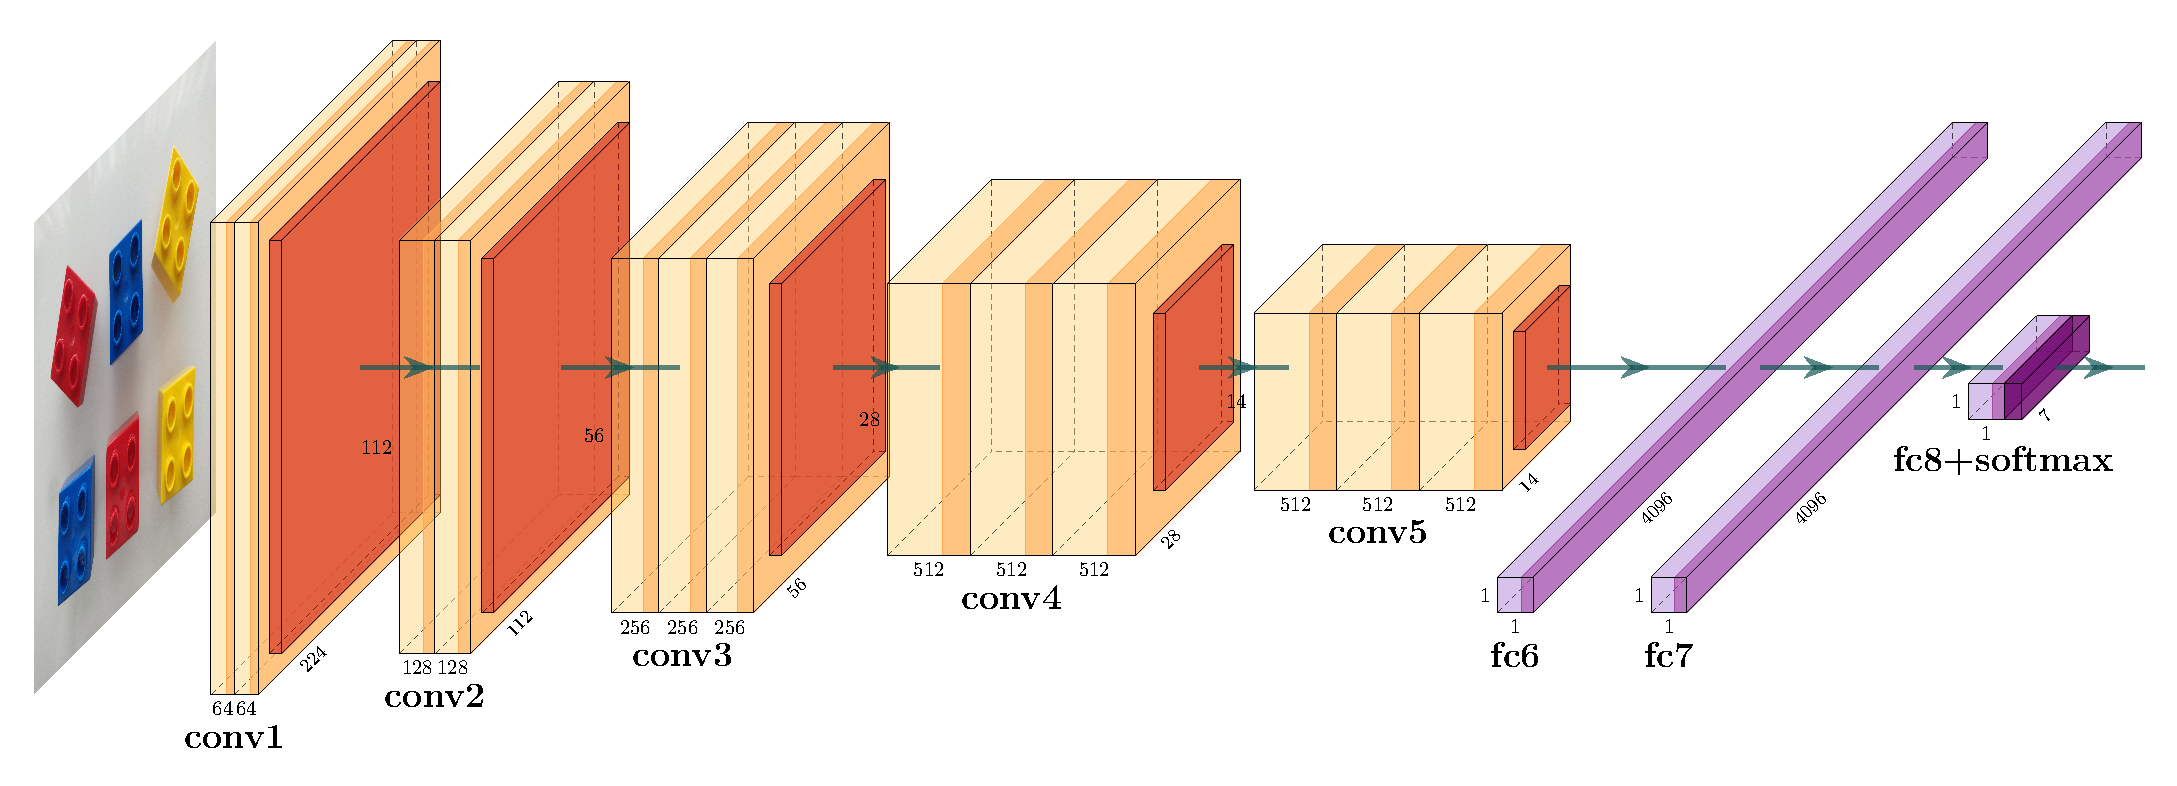
\includegraphics[width=1\textwidth]{Classificacion con redes neuronales/LEGO16.pdf}
	\caption{Estructura de LEGO16}
	\label{fig:LEGO16}
	\vspace{-5pt}
\end{figure}

\begin{figure}[ht]  %LEGO16 conv
	\centering
	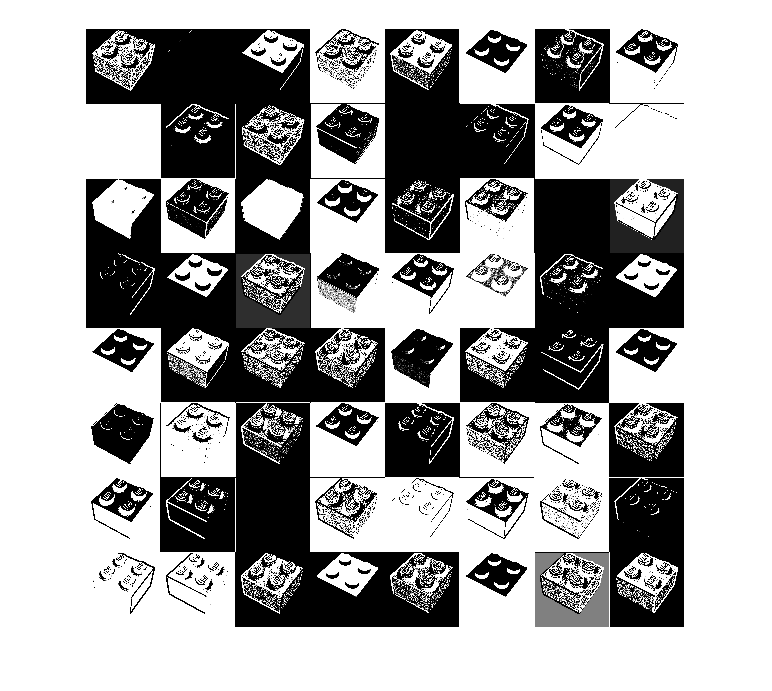
\includegraphics[width=0.8\textwidth]{Classificacion con redes neuronales/LEGO16_conv1.png}
	\caption{Activación de la primera convolución de LEGO16}
	\label{fig:LEGO16 conv}
	\vspace{-5pt}
\end{figure}


\subsection{Entrenamiento}
Con la ayuda de MATLAB y del conjunto de imágenes elaborado en \autoref{sec:Condiciones de entrenamiento} se ha reentrenado a VGG-16 para identificar 7 clases. Tras numerosas pruebas se han seleccionado las opciones de entrenamiento mostradas en la \autoref{tab:LEGO16 options}.

\begin{table}[ht]
  \centering
    \begin{tabular}{|l|c|}
    \hline
    \multicolumn{2}{|c|}{Opciones de entrenamineto} \\
    \hline
    Solver & \multicolumn{1}{l|}{Stochastic Gradient Descent with Momentum (SGDM)} \\
    \hline
    Momentum & 0.9 \\
    \hline
    Initial Learn Rate & 1.00E-04 \\
    \hline
    Learn Rate Schedule & piecewise \\
    \hline
    Learn Rate Drop Factor & 0.1 \\
    \hline
    Learn Rate Drop Period & 2 \\
    \hline
    L2Regularization & 0.004 \\
    \hline
    Max Epochs & 10 \\
    \hline
    Mini Batch Size & 16 \\
    \hline
    Shuffle data & every epoch \\
    \hline
    \end{tabular}%
  \caption{Opciones de entrenamiento de LEGO16}
  \label{tab:LEGO16 options}%
\end{table}%

\newpage
\subsection{Resultados}
Con la ayuda de MATLAB y de las bases de datos previamente comentadas, se va a realizar una evaluación del clasificador. En total se han empleado más de 3000 imágenes y a continuación se muestran los resultados obtenidos. Analizando estos resultados se puede obtener las tasas de aciertos y tasas de fallos (ver \autoref{fig:matriz LEGO16}).

Se puede realizar un estudio más intensivo analizando los verdaderos positivos y los falsos positivos (ver \autoref{fig:ROC LEGO16}). Este tipo de representación se conoce como curva \textit{ROC} (curva de característica operativa del recepto) y es ampliamente usada al evaluar clasificadores ya que permite mostrar de forma gráfica el comportamiento de la red. Otro dato importante de esta curva es el área que encierra, este dato es conocido como \textit{AUC} (Area Under the Curve). Este dato se puede ver en la \autoref{tab:ROC LEGO16}.

Las tasas de acierto y las \textit{AUC} obtenidas es bastante elevada si se tiene en cuenta el poco tiempo de entrenamiento. Si nos fijamos solo en los LEGOS observamos que los resultados son incluso mejores ya que solo ha habido un falso positivos y ninguna pieza mal identificada. Es decir, una tasa de falsos positivos es del 0.2\% y una tasa de acierto al identificar LEGOS del 100\%.

En general, este clasificador ha dado mejores resultados frente a LEGONet reduciendo los errores cometidos entre clases. Aunque, en la clase LEGO ambos han obtenido una tasa de acierto del 100\% pero LEGO16 ha conseguido reducir el número de falsos positivos. Probablemente se puedan obtener mejores resultados si se consigue entrenar durante más tiempo a la red, con más datos y con mayor VRAM. De esta forma se pueden evitar problemas por regularización aumentado el tamaño del \textit{batch}.

\begin{figure}[ht]  %Matriz LEGO16
	\centering
	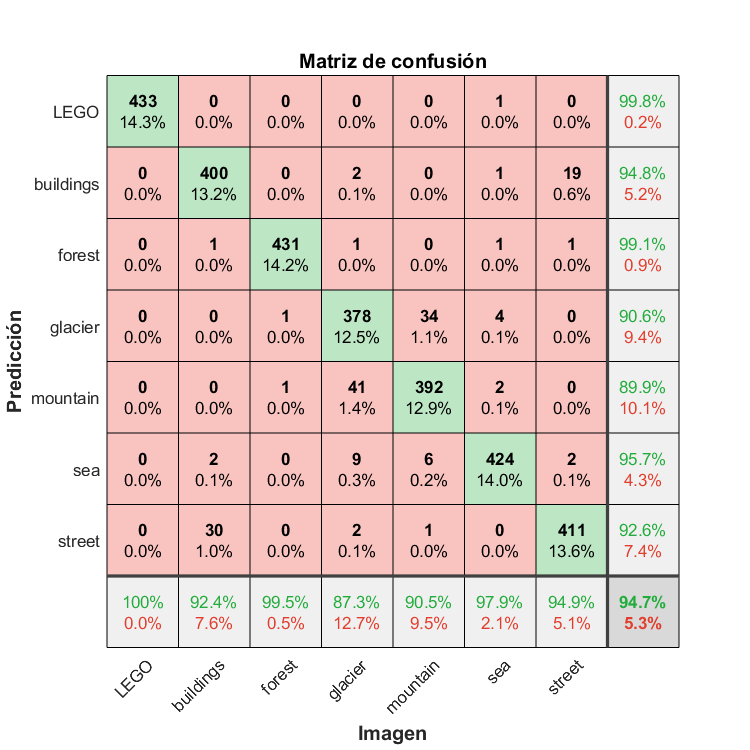
\includegraphics[width=0.8\textwidth]{Classificacion con redes neuronales/LEGO16_matriz.png}
	\caption{Evaluación de LEGO16: matriz de confusión}
	\label{fig:matriz LEGO16}
\end{figure}

\begin{figure}[ht]  %ROC LEGO16
	\centering
	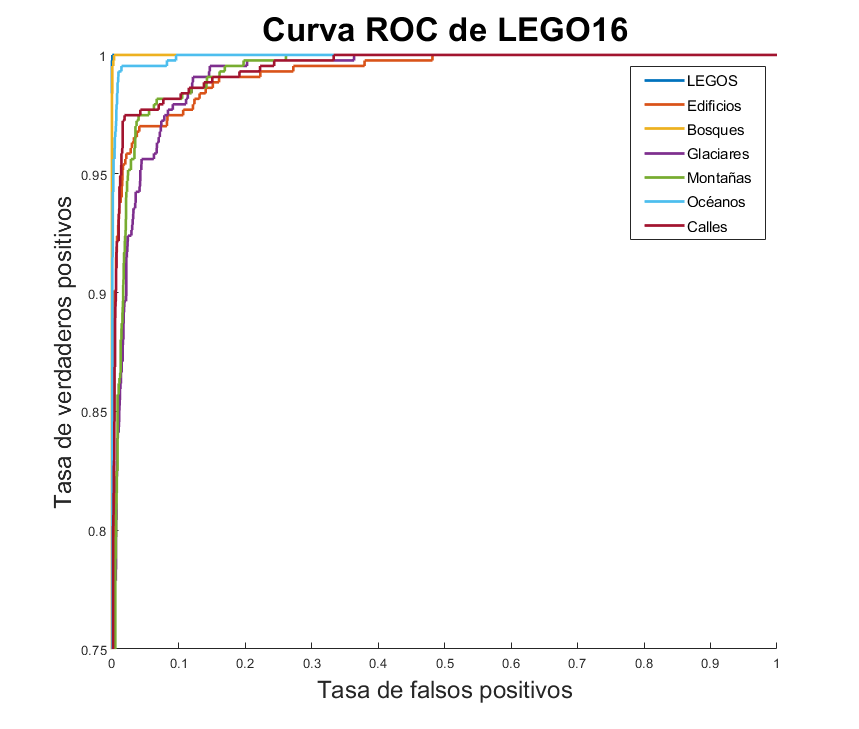
\includegraphics[width=0.8\textwidth]{Classificacion con redes neuronales/ROC2 LEGO16.png}
	\caption{Evaluación de LEGO16: curvas \textit{ROC}}
	\label{fig:ROC LEGO16}
\end{figure}

\begin{table}[ht]
  \centering
    \begin{tabular}{|l|r|}
    \hline
    \multicolumn{2}{|c|}{\textit{AUC}}\\
    \hline
    LEGOS & 1.00 \\
    \hline
    Edificios & 0.9927 \\
    \hline
    Bosques & 1.00 \\
    \hline
    Glaciares & 0.9910 \\
    \hline
    Montañas & 0.9928 \\
    \hline
    Océanos & 0.9992 \\
    \hline
    Calles & 0.9946 \\
    \hline
    \end{tabular}%
    \caption{Evaluación de LEGO16: áreas encerradas debajo de la curva \textit{ROC} para cada clase}
  \label{tab:ROC LEGO16}%
\end{table}%
